\documentclass[12pt, addpoints]{exam/exam}

\usepackage{hyperref}
%\usepackage{mdframed}
\usepackage{graphicx, caption}	
%\usepackage{array, multicol, tabu}
\usepackage{amsmath, amsthm, amssymb}
\usepackage{comment}
\usepackage{enumitem}
\usepackage{url}
\usepackage{textcomp}
\usepackage{wrapfig}
\newcommand{\1}{^{-1}}
\newcommand{\vect}[1]{\mathbf{#1}}
\newcommand{\R}{\mathbb R}
\newcommand{\vstr}{\vspace{\stretch{1}}}
\everymath{\displaystyle}
\setlength{\parindent}{0pt}

\theoremstyle{plain}
\newtheorem{thm}{Theorem}
\newtheorem*{thm*}{Theorem}

%\printanswers
\pointformat{\bf(\thepoints)}
\pointpoints{pt}{pts}
\bonuspointformat{\bf(\thepoints)}
\bonuspointpoints{pt}{pts}

\coverfirstpageheader{\bf MATH 235 (Calculus I) \\
		Fall 2017 \\
		}
		{}
		{{Name:} \underline{\hspace{40ex}} \\
		\vspace{0.5pc}
		Thurs 26 Oct 2017}
\coverextraheadheight[2pc]{0in}
\coverfirstpagefooter{}{}{\Large Good luck!}
\coverrunningheader{}
	{Exam 2: Derivatives, with story problems}
	{}
\coverrunningheadrule	
\coverrunningfootrule
\coverrunningfooter{Calc I Fall 2017}{}{p. \thepage\ (of \numpages)}

\firstpageheader{}
	{Exam 2: Derivatives, with story problems}
	{}
\firstpageheadrule
\firstpagefootrule
\firstpagefooter{Calc I Fall 2017}{}{p. \thepage\ (of \numpages)}

\runningheadrule
\runningheader{}
	{Exam 2: Derivatives, with story problems}
	{}
\runningfootrule
\runningfooter{Calc I Fall 2017}{}{p. \thepage\ (of \numpages)}

\title{\vspace{-8pc}
\vfill{\Huge
	\bf Exam 2: Derivatives, with \\ story problems %\\ 
	(\S2.1, 2.7-3.9)} 
	}
%\author{}
\date{}

% % % % % % % % % % % % % % % % % % % %
\begin{document}

\begin{coverpages}
\maketitle
\thispagestyle{headandfoot}
\vspace{-4pc}
{\bf Exam Instructions:} You have 75 minutes to complete this exam.  Justification is required for all problems.  Notation matters!  You will also be penalized for missing units and rounding errors.  
No electronic devices (phones, iDevices, computers, etc) except for a \textbf{basic scientific calculator}.  On story problems, round to two decimal places. 

\vspace{1pc}
If you finish early then you may leave, UNLESS there are less than 5 minutes of class left.  To prevent disruption, if you finish with less than 5 minutes of class remaining then please stay seated and quiet.

\begin{flushright}
%In addition, please provide the following data:

\vspace{0.3in}
%Drill Instructor: \underline{\hspace{40ex}}

\vspace{0.3in}
%Drill Time: \underline{\hspace{40ex}}
\end{flushright}

\vfill
\textbf{Your signature below indicates that you have read this page and agree to follow the Academic Honesty Policies of James Madison University.}  

\vspace{0.3in}
Signature: {\bf (1 pt)} \underline{\hspace{73ex}}

% % % % % % % % % %
\newpage
\vspace*{\fill}
\gradetable
%\textbf{Formulas you may need:}
%\vspace{-2pc}
%\begin{center}
%\vspace*{\fill}
%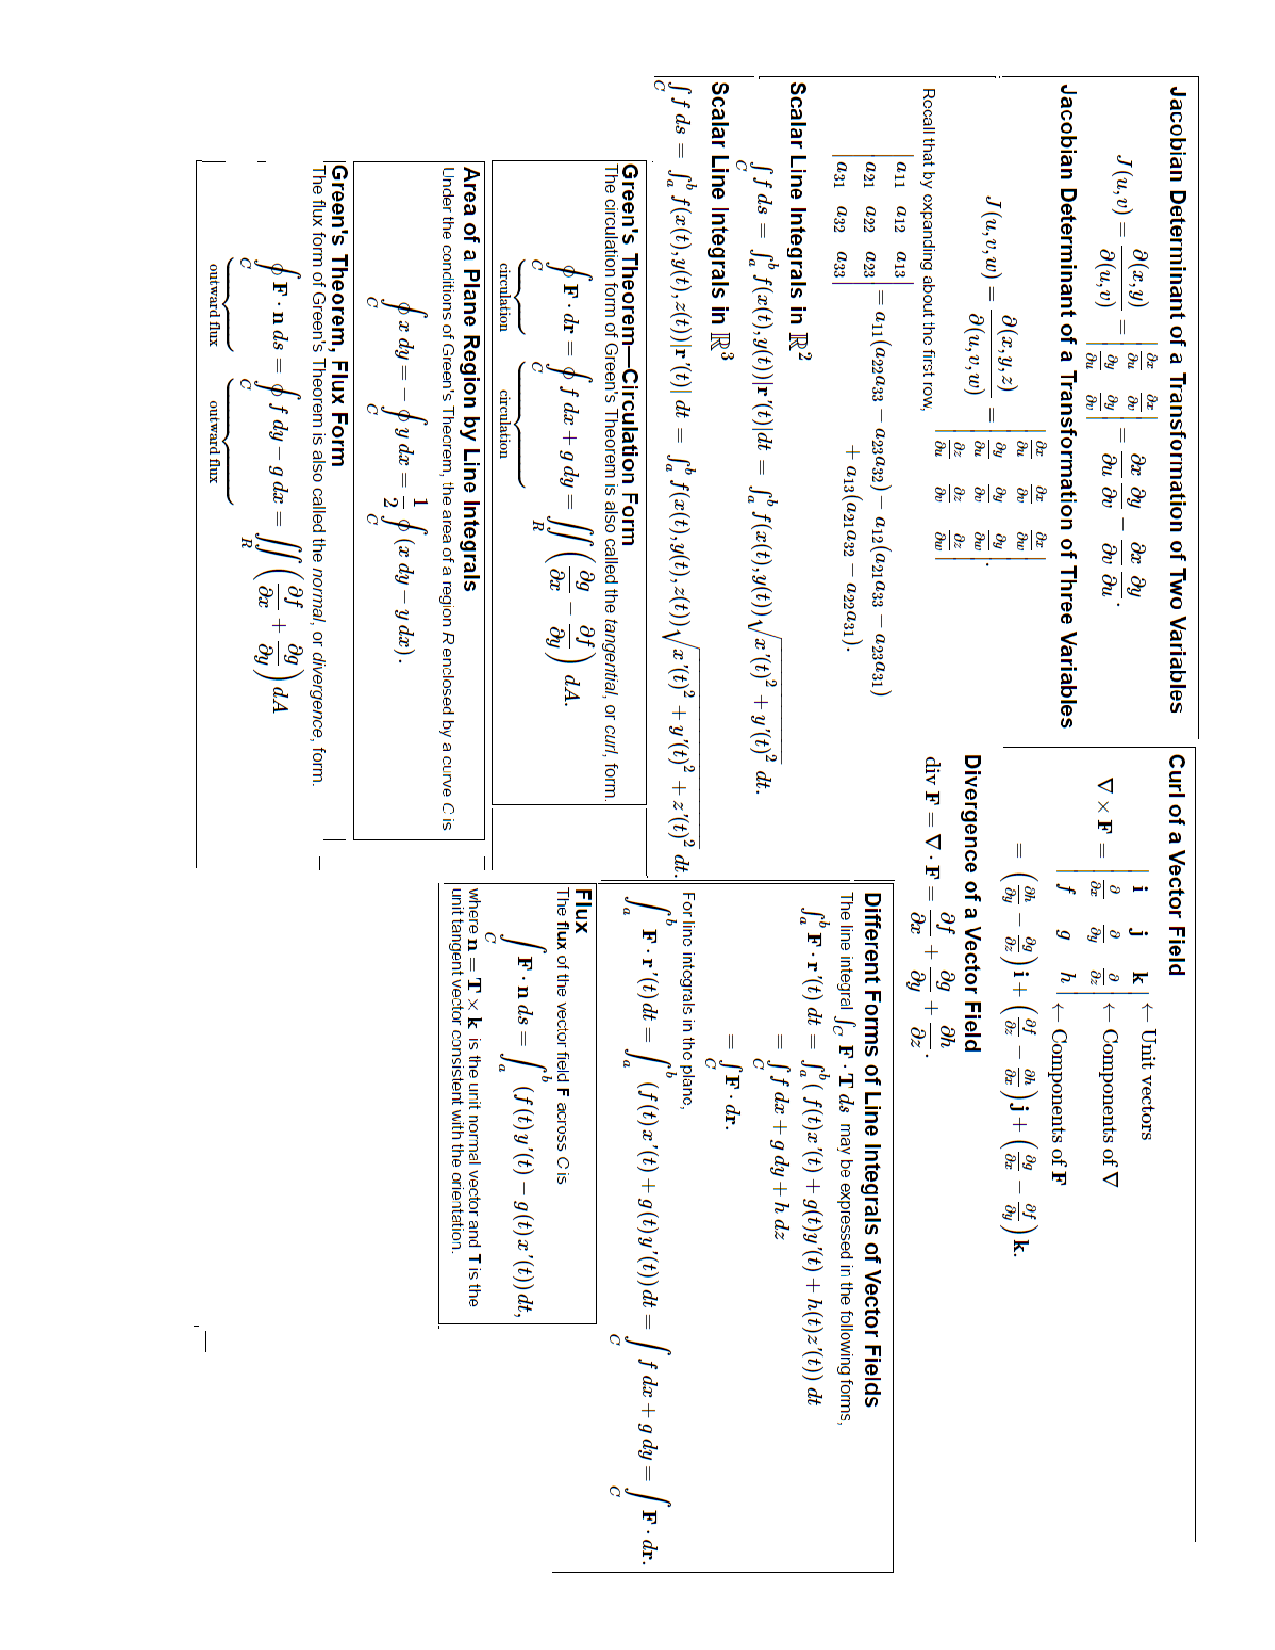
\includegraphics[scale=0.84]{Exam3FormulaSheet.pdf}
%\vspace*{\fill}
%\end{center}
\end{coverpages}

% % % % % % % % % % % % % % % % % % % %
\begin{questions}
\thispagestyle{headandfoot}

% % % % %
\question[15] %{\bf 3.9 \#42} 
Two carts, A and B, are connected by a rope 39 %29
 ft long that passes over a pulley $P$ (see the figure).
\vspace{-0.9pc}
\begin{center}
	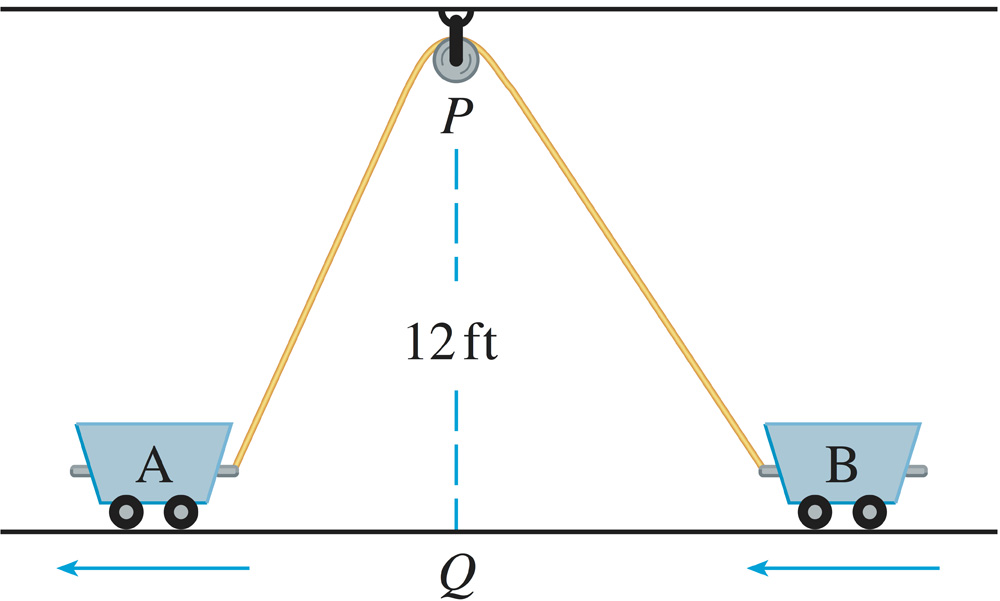
\includegraphics[scale=4.1]{3-9_42Stewart8Ed.jpg}
\end{center}
\vspace{-0.9pc}

The point $Q$ is on the floor 12 ft directly beneath $P$ and between the carts.  Cart A is being pulled away from $Q$ at a speed of 2 %1 
ft/s.  How fast is cart B moving toward $Q$ at the instant when cart A is 5 ft from $Q$?

\vfill

\newpage
% % % % %
\question %{\bf 2.7 \#18} 
The graph of the function $f$ is shown below.
%\vspace{-0.5pc}
\begin{center}
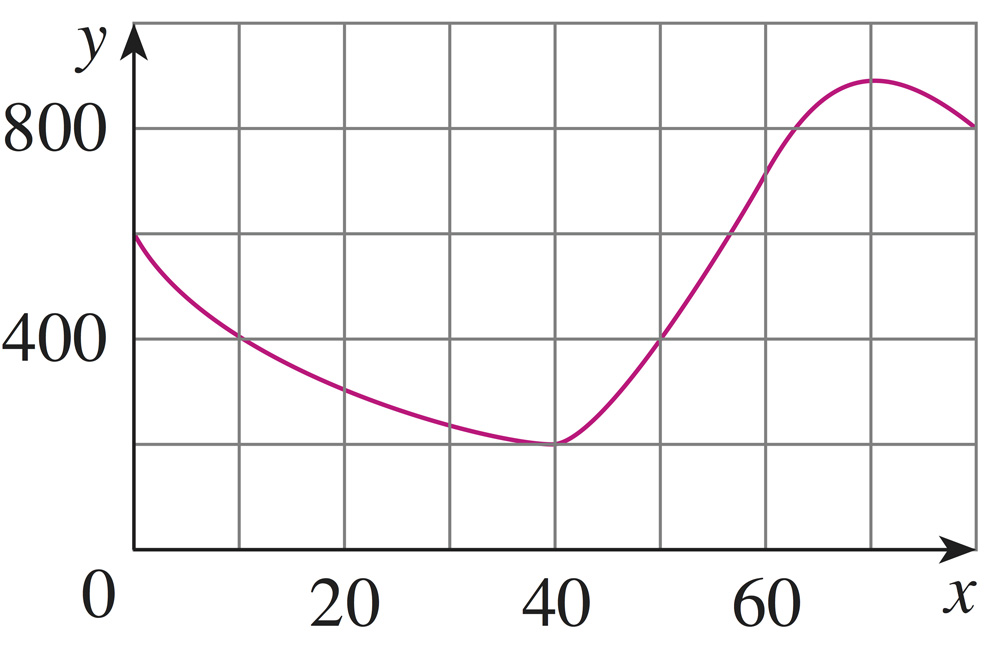
\includegraphics[scale=4.5]{2-7_18Stewart8Ed}
\end{center}
%\vspace{-0.5pc}
	\begin{parts}
	\part[4] Find the average rate of change of $f$ on the interval $[20,60]$%$[0,40]$
	.
	\vfill
	
	\part[4] Identify an interval on which the average rate of change of $f$ is 0.
	\vfill
	
	\part[4] Which interval gives a larger average rate of change, $[40,60]$ %$[0,40]$ 
	or $[40,70]$%$[10,40]$
	?  How can you tell?
	\vfill
	
	\part[4] Compute $\frac{f(40)-f(10)}{40-10}$%$\frac{f(50)-f(20)}{50-20}$
	; what does this value represent geometrically?
	\end{parts}
	
\vfill	

\newpage
% % % % %
\question[15] %{\bf \S2.8 \#30} 
Use the \textbf{limit definition} of the derivative to differentiate the function $y=(2x+1)^3$.  You will be penalized for incorrect notation.
%\vspace{22pc}

\newpage
% % % % %
\question[10] %{\bf CR \#30}
Find $y'$, given $y=\frac{(x^2+1)^4}{(2x+1)^3(3x-1)^5}$%$y=\frac{(x^2+1)^3}{(2x+1)^5(3x-1)^4}$
.
\vfill

\question[10] %{\bf 3.3 \#42} 
Evaluate $\lim_{\theta\to 0}\frac{\cos{\theta}-1}{\sin{\theta}}$.	
\vfill

\newpage
% % % % %
\question %{\bf 3.8 \#18} 
The temperature of an object whose surroundings are temperature $T_s$ is given by
\[
T(t)=(T(0)-T_s)e^{kt}+T_s,
\]
where $k$ is some constant.  \textbf{Newton's Law of Cooling} says the change in temperature at time $t$ is proportional to the difference between the temperature at time $t$ and the surrounding temperature. 
\begin{parts}
	\part[8] Find $\frac{dT}{dt}$.  Then rewrite your answer in terms of $T(t)$. 
	\vspace{8pc}
	
	\part[10] A freshly brewed cup of coffee has temperature 95%105
	$^{\circ}$C in a 20%30
	$^{\circ}$C room.  When its temperature is 70%80
	$^{\circ}$, it is cooling at a rate of 1$^{\circ}$C per minute.  When does this occur?  \textit{Hint: To solve for $k$, you must write your answer to part (a) in terms of $T(t)$.  If you don't, then you will have an equation that cannot be solved by hand.}
	
	\end{parts}
	
\newpage
% % % % %
\question[15] %{\bf 3.7 \#36} 
Invasive species often display a wave of advance as they colonize new areas.  Mathematical models based on random dispersal and reproduction have demonstrated that the speed with which such waves move is given by the function 
\[
f(r)=2\sqrt{Dr},
\]
where $r$ is the reproductive rate of individuals and $D$ is a parameter quantifying dispersal.  Calculate the derivative of the wave speed with respect to the reproductive rate $r$ and explain its meaning.

	
%\newpage
% % % % %
%\question \begin{parts}
%	\part {\bf 3.4 \#72} If $g$ is a twice differentiable function and $f(x)=xg(x^2)$, find $f''$ in terms of $g$, $g'$, and $g''$.
%	\vspace{22pc}
%	
%	\part {\bf 3.4 \#74} If $F(x)=f(xf(xf(x)$, where $f(1)=2$, $f(2)=3$, $f'(1)=4$, $f'(2)=5$, and $f'(3)=6$, then find $F'(1)$.	
%	\end{parts}
%	
%\vfill	


%\newpage	
% % % % %
%\question[] {\bf 3.7 \#12} \begin{parts}
%	\part Sodium chlorate crystals are easy to grow in the shape of cubes by allowing a solution of water and sodium chlorate to evaporate slowly.  If $V$ is the volume of such a cube with side length $x$, calculate $\textstyle\frac{dV}{dx}$ when $x=$3 mm and explain its meaning.
%	\vspace{22pc}
%	
%	\part Show that the rate of change of the volume of a cube with repsect to its edge length is equal to half the surface area of the cube.  Explain geometrically why this is true.
%	\end{parts}
%
%\vfill


\end{questions}

\end{document}